\chapter{Components: `The Flux Capacitor' for Pipete-Based Laminar Flow Patterning}

\section{Preface}
Contents of this chapter are taken from \cite{Berthier:2011fk} which was written in equal part with Erwin Berthier.

\section{Introduction}
Laminar flow patterning (LFP) is a prominent and established method used in microfluidics to pattern cells, particles, and treatments within a single channel \cite{Takayama:1999qf}. The method can be used to precisely control the nature and location of an interface between two miscible or non-miscible fluids, without requiring a physical divider \cite{Lucchetta:2005kn}. In addition, the laminar behavior of fluids at the microscale allows diffusion to be leveraged as a highly controllable mixing force enabling the creation of precise gradients within a microchannel \cite{Sia:2003bh}. The method has also been leveraged in areas such as the dynamics of chemical and enzymatic reactions \cite{Regenberg:2004ly} and the response of cell cultures to patterned treatments \cite{Tourovskaia2005Differentiation}. LFP has proven to be an enabling method for microfluidic cell-based assays where it is predominantly used for generating gradients of soluble factors in chemotaxis assays \cite{Li-Jeon:2002uz}, but is also used in the study of soluble factor signaling between different cell compartments \cite{Torisawa:2009bh,Sung:2010fk}, and for patterning a gap between two cell culture populations in wound-healing/invasion assays \cite{Wong:2008lq}.

\begin{figure}[!b]
\centering
  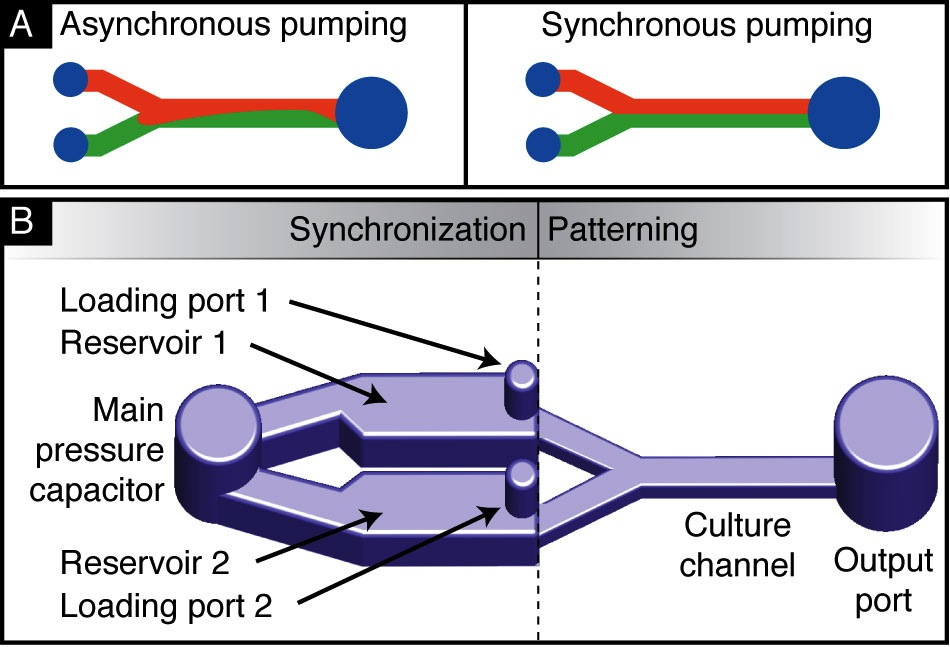
\includegraphics[width=8cm]{figure1.jpg}
  \caption{\textbf{The flux capacitor}. A. Flow pattern in a laminar flow patterning channel with unsynchronized pressures (left) and synchronized pressures (right). B. Schematic of the proposed synchronization method. A fluidic capacitor links the two sample loading ports of the Y-channel. The capacitor acts as a temporary destination for loaded fluid and balances the pressure applied to each branch for laminar flow patterning.}
  \label{fig:scematic}
\end{figure}

Despite the multitude of applications demonstrated using LFP, use of the method has not spread further than a restricted number of microfluidic labs, especially for applications where only a brief period of laminar flow is needed (\emph{i.e.}, in short-term LFP applications such as transient gradients or cell patterning). In short-term LFP applications, the complexity and expertise required to connect and operate syringe pumps for a brief period of laminar flow is prohibitive compared to alternative approaches. Further, tight control over flow rates is required to maintain synchronization of the flow through each branch. Using syringe pumps and tubes, it is difficult to ensure that flow through each branch ceases at exactly the same time due to different flow relaxation times caused by upstream capacitance and pumping mechanics (Fig \ref{fig:scematic}A). Other difficulties of working with tubing include dead-volumes and air bubbles \cite{Paguirigan:2008xe}. Thus, ease-of-use and accessibility are the biggest barriers to wide-spread use of short-term LFP for the purpose of cell patterning and transient gradients. A passive method to perform LFP using capillary action has been demonstrated \cite{Kim:2005fk} previously but requires the use of surface patterning and surfactants which increase the fabrication complexity and prevent its use in cell-based applications. 

We describe here a passive microfluidic device, sometimes called `The Flux Capacitor', that requires only a single pipette to operate and addresses the challenge of manually synchronizing flows for LFP. One half of the device is a typical branched channel for LFP. The other half, placed upstream, consists of synchronization components that  provides an intermediate storage location for sample fluids and a unified pressure source. We achieve this by using reservoir channels and a surface tension-based fluid capacitor. These elements maintain constant fluid interfaces within the patterning area throughout sample loading. Specifically, the ability to cease flow down each branch at exactly the same time to preserve patterning is a major advantage of this method. The synchronization components can be used to stabilize LFP when using syringe pumps but the components also enable the use of other pumping strategies such as surface-tension base pumping \cite{Walker:2002ez}. In the case of surface-tension-based pumping, sample droplets can be placed using a pipette in any order and at any time relative to one another using a standard micropipette without disturbing the patterned interfaces.

%The robust, pipette-based LFP method is particularly well-suited for patterning cell populations in close proximity and would find immediate utility in co-culture and wound-healing assays. Non-adhesion-based methods for patterning in microscale culture applications have been demonstrated before but typically rely on the use of channel constrictions or membranes to help segregate each cell population during seeding and subsequent culture \cite{Domenech:2009jt}. Such geometries result in diminished transport of soluble factors between the compartments, reducing the potential sensitivity of the co-culture assay. The method presented here alleviates the need for these constrictions, increasing the diffusive flux between the cell populations, and therefore the sensitivity and efficiency of co-culture assays.

The robust, pipette-based LFP method is particularly well-suited for patterning cell populations in close proximity and would find immediate utility in co-culture and wound-healing assays. In order to characterize the functional range of the proposed method, numerical simulations were performed to understand the impact of different design considerations. Experimental demonstrations are used to illustrate the operation and potential applications of this method. Finally, a three-flow device was used to pattern two different cell populations separated by a tunable gap as a means of modulating cell-cell communication. %Finally, given the limited use and inaccessibility of LFP for co-culture in the past, a brief comparison with other microfluidic segregated co-culture methods is provided to highlight some fundamental advantages. 

\section{Methods}

\subsection{Numerical Simulations}

To better understand device operation, numerical modeling was performed using an electrical analogy of the microfluidic device that is valid for low Reynolds number laminar flows (Figure \ref{fig:modeling}A). Simulations were performed using matlab with a time step of 0.1 ms and recorded for two different durations to characterize the beginning and ending of the flow (Fig \ref{fig:modeling}). The resistance of each channel is calculated using the Washburn law while pressure drops at channel turns and junctions are neglected. Ports are modeled as non-ideal capacitors with a volume-pressure relationship given in Eq \ref{eq:laplace}. The modeled device consists of two input ports of radius 500 $\mu$m, a main capacitor port of radius 1.25 mm and an output port of radius 1.5 mm. The reservoir ports are 250 $\mu$m tall, 4mm long and 2 mm wide. Each small branch of the Y channel is 100 $\mu$m tall, 750 $\mu$m wide, and 3 mm long and join into a channel that is 100 $\mu$m tall, 1 mm wide, and 5 mm long. 

\subsection{Device Fabrication}The device is made by bonding a PDMS (poly-dimethylsiloxane) mold of the channel network fabricated using standard softlithography techniques to a glass slide \cite{Jackman1998Fabricating-lar}.  Plasma treatment of the PDMS and the glass was performed to render the surfaces hydrophilic and enable capillary filling of the device using PBS applied to each of the large ports. Initial filling can also be achieved using vacuum filling\cite{Zhao:2009uq} or by filling initially with ethanol and immediately replacing with PBS or media.

\subsection{Device Characterization}

The device is filled with PBS such that the fluid is roughly flush with the surface of the device. A volume of 2.5 $\mu$ L was used to load samples. Samples were loaded with a minimum of a 3 second interval between each addition. PBS with red and green food colorant was used to illustrate device operation (Fig \ref{fig:experimental1}). Imaging of the device was performed on an Olympus SZX12 stereoscope (Olympus, Center Valley, PA). Similarly fluorescent analysis was performed using Alexa488 dye (Molecular Probes, Carlsbad, CA). 

\subsection{Cell culture}

Cell lines (MCF7-GFP, MCF7-RFP, BEAS-2B, LNCaP and MC3T3-E1) were cultured according to the ATCC guidelines. At 80\% confluency, the cell cultures were detached using trypsin, centrifuged and resuspended in PBS at 3.$10^{6}$ cells / mL. For 3-D applications, a cell suspension at a final concentration of 3.$10^{6}$ cells / mL was achieved by mixing 1:4 parts of collagen type I stock solution at 8 mg/mL, 1:4 parts of HEPES buffer and 1:2 parts of cell suspension at 6.$10^{6}$ cells / mL.

\subsection{Cell patterning}

A device was fabricated with three sample inputs to allow a cell-free solution to be patterned between two outer streams containing cells. Two MCF7 cell lines (ATCC), one expressing GFP (green fluorescent protein) and the other RFP (red fluorescent protein) were flown in the two outmost channels, green on one side and red on the other. Burst image acquisition was performed to record a movie of the actual loading process (Fig \ref{fig:experimental2}B). Bone marrow MC3T3-E1 cells and LNCaP prostate cancer cells were flown in a similar manner in 3-D collagen suspension (Fig \ref{fig:experimental2}D). In this case, the device was pre-filled with collagen to provide uniform viscosity for loading of the collagen-cell suspension. The migration of the bone marrow cells was observed in 2-D at 24 and 48 hours in the presence or absence of the LNCaP cells (Fig \ref{fig:cocultureData}B). Finally a wound healing-like assay was performed by patterning two compartments of lung epithelial cells, BEAS-2B, after coating with bovine collagen, and images were recorded at 24 and 48 hours.


\section{Results and Discussion}

\subsection{Demonstration of Laminar Flow Patterning}

The device used in this demonstration consists of a basic Y-channel with additional components to synchronize flows (Fig \ref{fig:scematic}B). Each branch of the Y-channel contains a port to load the fluid of interest and a reservoir channel to hold that fluid temporarily. All reservoirs are connected to a central capacitor port that charges with fluid when samples are inserted into the input ports (Fig \ref{fig:experimental1}). Rapid charging of the capacitor occurs due to the low resistance between the inputs and capacitor and ensures that an equal pressure is applied on each branch of the Y channel. By applying an equal pressure to each branch, the proportion of fluid that travels down each branch is determined by their fluidic resistance. Thus, a loading event at any input, at any point in time, causes the contents of each reservoir to be pushed downstream in accordance with the ratio of each path resistance and results in LFP with a steady fluid interface.

Fig \ref{fig:experimental1}B demonstrates the steady flow-interface produced throughout pumping using colored fluids. This example also shows that the samples do not need to be loaded simultaneously for robust patterning. This is particularly beneficial in the context of a biology lab where the user often handles a multitude of reagents\slash solutions\slash dilutions. Fig \ref{fig:experimental1}C shows that branch resistances can be altered to adjust the location of the flow interface (2:1 flow ratio between branches). Similar experiments using fluorescent dye illustrate a well-defined flow interface and are summarized in the images of Fig \ref{fig:experimental1}D.
\begin{figure}[!t]
\centering
  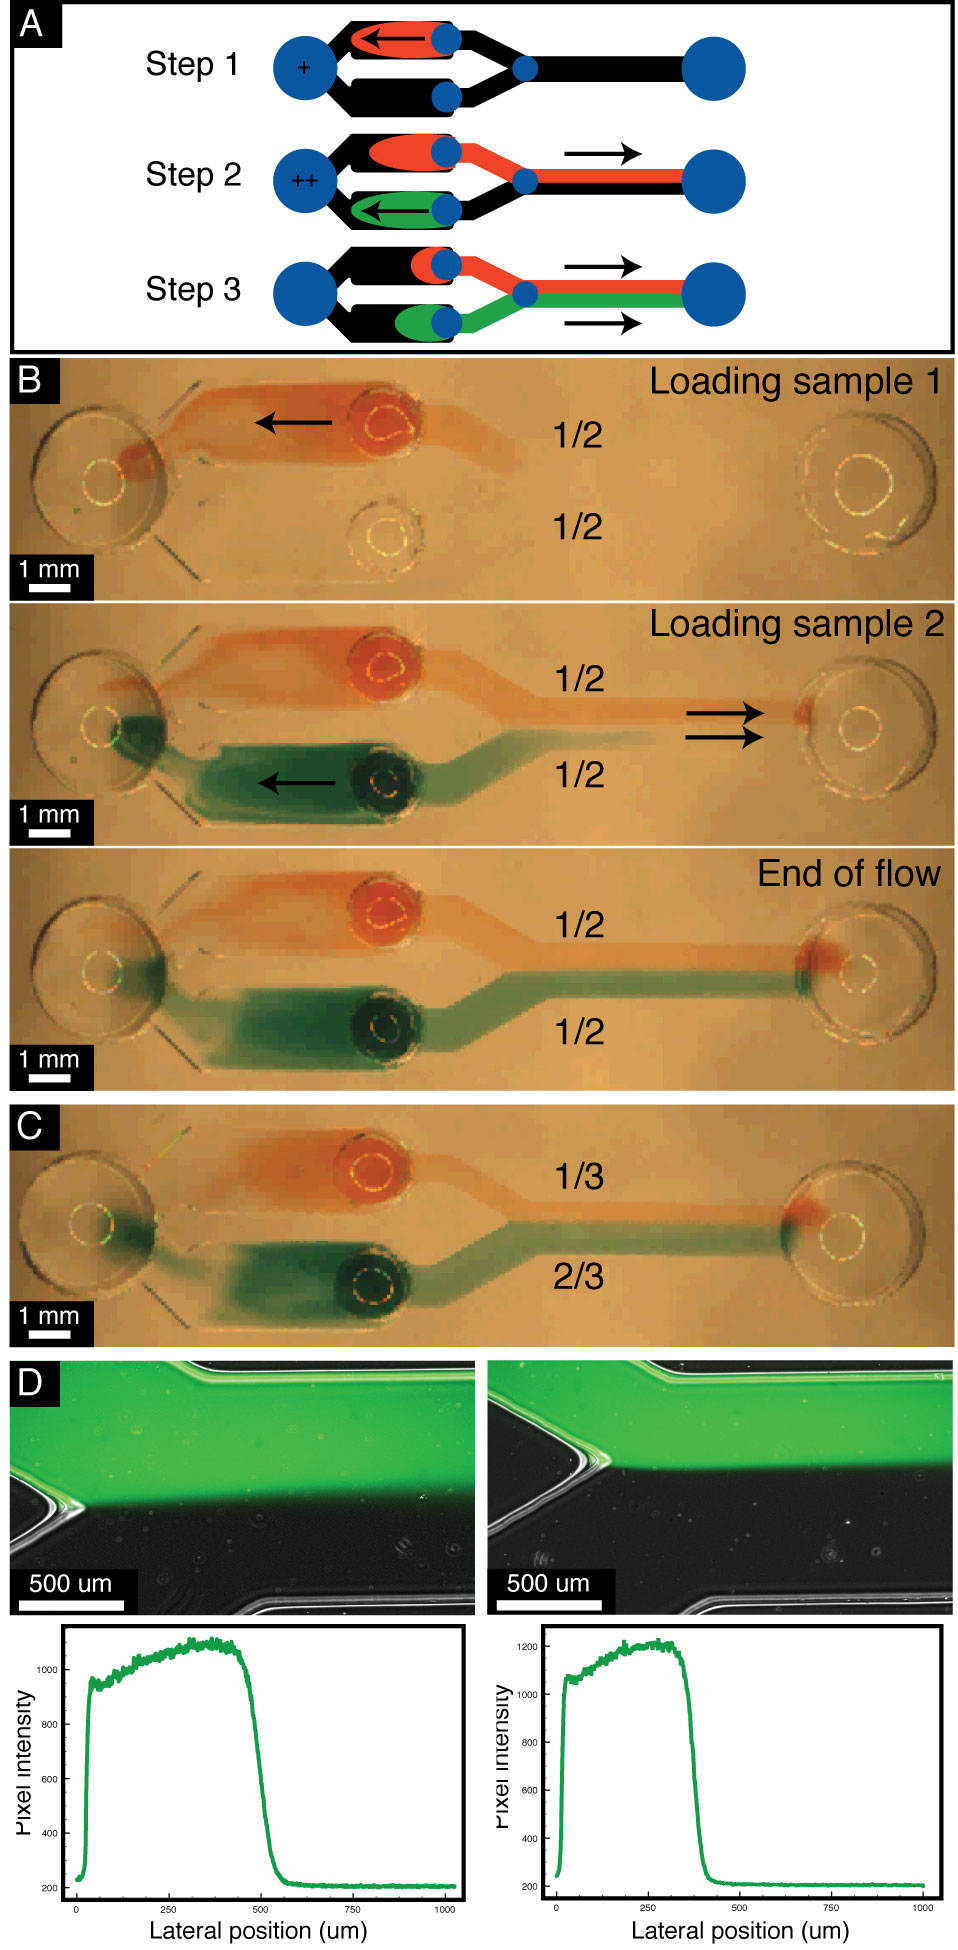
\includegraphics[width=8cm]{figure2.jpg}
  \caption{\textbf{Experimental validation of pipette-based LFP}. All sample fluids were added with a minimum of 3 seconds between each event. A. Simple three step description of the loading protocol. B. Three frames picturing a channel with equal ratio patterning at different time-points of the process. C. Image at the end of the flow in a channel designed to split the culture channel into 1/3 and 2/3 sections. D. Fluorescent and bright field merged images of Alexa488 dye flow in the 1/2-1/2 patterning device (left) amd the 1/3-2/3 device (right) and a the respective cross section fluorescent intensity profile. }
  \label{fig:experimental1}
\end{figure}

\subsection{Analysis of Each Device Component}

Analytical and numerical modeling have been performed to better understand the contribution of the different components of the microfluidic device. In order to adapt the use of this method to other applications, each component and the design considerations required for its proper function are discussed. \\

{\bf Surface tension and port capacitors.} The fluid-air interface formed by a port can be used as a capacitor in a fluidic circuit, having a pressure-volume relationship. The surface tension-generated pressure, $P_{port}$, in a droplet of curvature $R_{curv}$, at each port acts as a capacitor of fluid according to the Laplace relationship shown in Eq \ref{eq:laplace} where $\gamma$ is the surface tension of the fluid. The volume of liquid, $V$, contained in a port, can also be linked to the radius of curvature using Eq \ref{eq:volumeSphericalCap}. Eq \ref{eq:laplace} and Eq \ref{eq:volumeSphericalCap} establish a pressure-volume relationship that defines the capacitor. For instance, a large port will be able to contain a large volume of fluid and will act as a weak capacitor, whereas a small port will act a stiffer capacitor generating large pressures when fluid is added. 

\begin{equation}
P_{port} = \frac{2\gamma}{R_{curv}}
\label{eq:laplace}
\end{equation}

\begin{equation}
V = \frac{\pi}{3} (2R_{curv}^{3} - (R_{curv}^{2} - a^{2})^{1/2} (2R_{curv}^{2} - a^{2}) )
\label{eq:volumeSphericalCap}
\end{equation}

As seen in Fig \ref{fig:scematic}B, small ports (low-volume, stiff capacitors) are used for the loading ports of the device while large ports (high-volume, weak capacitors) are used to link the inputs and act as low pressure points for the fluidic circuit. Each large port is made big enough to absorb the whole amount of liquid that will be inserted for patterning. The loading ports are made small enough to quickly drive fluid to the capacitor and reduce synchronization times (Fig \ref{fig:modeling}). \\

\begin{figure}[!t]
\centering
  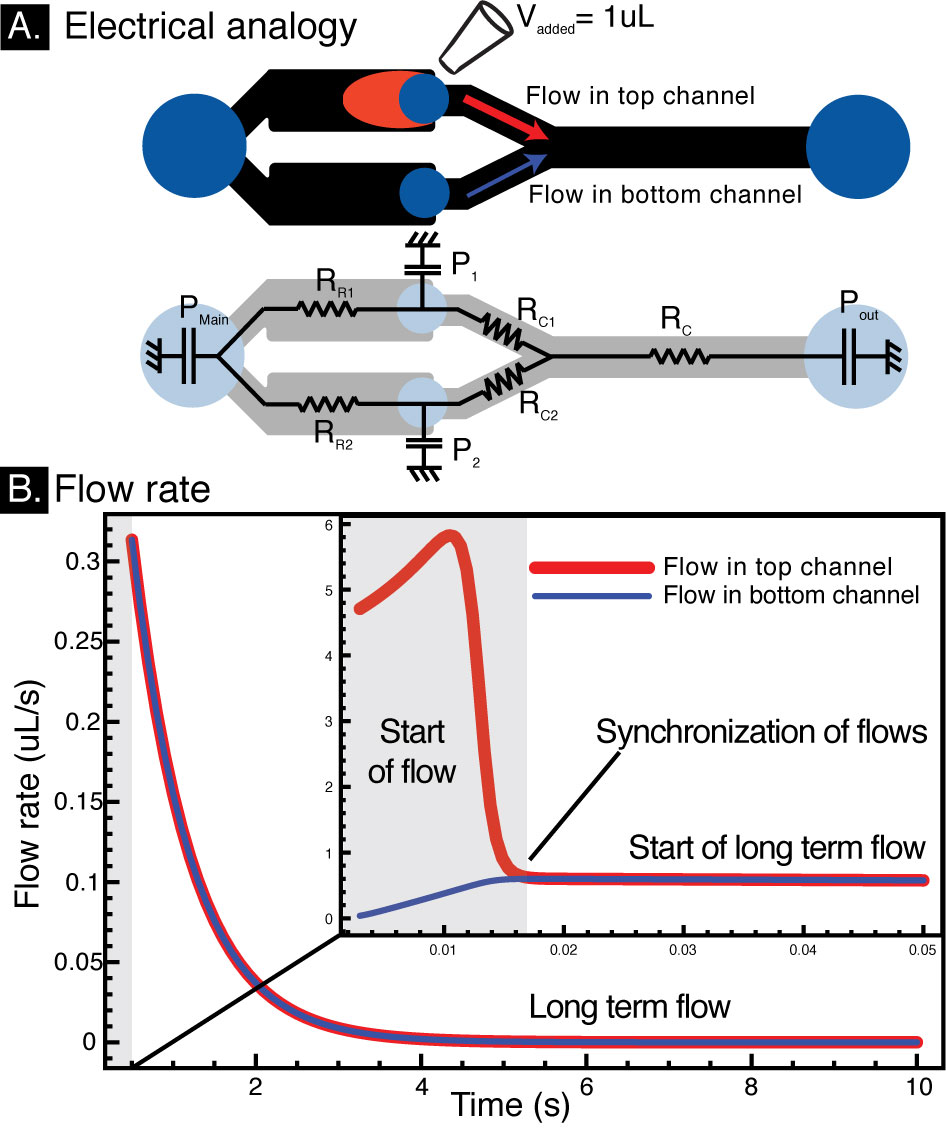
\includegraphics[width=8cm]{figure3.jpg}
  \caption{\textbf{Flux capacitor operation}. A. Electrical circuit analogy used for the numerical simulation. The different passive pumping ports can be modeled as capacitors. B. Flow rate vs. time in the each branches of the Y channel. Port pressures begin at different values, resulting in imbalanced flow rates. Within 15 ms port pressures equilibrate, leading to synchronization of the flows in both branches of the ``Y''. }
  \label{fig:modeling}
\end{figure}

{\bf Synchronization of the flow.} The experimental results of Fig \ref{fig:experimental1} show that laminar flow patterning is maintained throughout pumping. However, a short-lived disturbance of the flow pattern occurs upon each addition of fluid to an input port, which is difficult to identify in the images. The disturbance results from the short amount of time it takes for the capacitor to be charged. Simulations performed to characterize the transient flow profile in each branch of the Y-channel after adding a single droplet of 1.0 $\mu$ L in one of the input ports show that synchronization of the flows occurs in 15 ms (Fig \ref{fig:modeling}B). During the rest of the flow (4 s) the flows in both branches of the Y channel match. An additional drop can be applied to any port at anytime (before or after the flow stops), causing the process of synchronization described here to be repeated. Shorter synchronization times minimize the time that flows are imbalanced and can be achieved by reducing the radius of the sample loading port, decreasing the volume being loaded, and reducing the resistance of the reservoir channels. \\

{\bf Reservoir channel design.} The reservoir channels keep samples from mixing in the capacitor port. If the samples are allowed to reach the capacitor, samples might mix or possibly travel down an alternate branch of the device. Thus, the reservoir channels must be able to accommodate the entire sample volume. Based on previous characterizations of flow in rectangular channels, the amount of fluid needed to go beyond the end of the reservoir, $V_{overfill}$, is at most 0.48 times the volume of the reservoir due to parabolic flow profiles (Eq \ref{eq:volumeError2}) \cite{Warrick:2007lq}. Using this piece of information, the length of the reservoir channel can be designed appropriately. \\

\begin{equation}
V_{overfill} \ge 0.48 \, V_{channel}
\label{eq:volumeError2}
\end{equation}

{\bf Y channel design.} The ratio of flow down each branch of the Y-channel after synchronization, $Q_{1}/Q_{2}$, is proportional to the ratio of the resistances of each branch, $R_{C2}/R_{C1}$. Although the primary function of the branches is to determine where the interface between the flows will be patterned, they must also be designed to allow enough time for synchronization (Fig \ref{fig:modeling}B). As mentioned previously, the Y-channel has a significantly higher resistance than the reservoirs such that when fluid is added to a loading port, most of the fluid travels directly to the capacitor port, charging it with fluid. Channel dimensions can be reduced to pattern narrower regions of interest (50-100 $\mu$m) and would result in longer pumping times. The pumping mechanism can be scaled to increase pumping velocities to avoid cell settling during patterning.\\

%{\bf Sample loading.} The timing of the loading no longer influences patterning but can affect how much sample is left in each reservoir channel after patterning. In the case of symmetric patterning, after the first sample is loaded and comes to rest, half of the sample will remain in the reservoir channel. After loading the second sample in the other port, the remainder of the first sample will be pushed out of its reservoir channel and half of the second sample will remain in its reservoir. Alternatively, if the loading of the first and second sample had been perfectly synchronized, none of either sample would remain in the reservoir channels. %Both cases result in symmetric patterning but have different amounts of sample left over in the reservoir channels. Furthermore, this illustrates that a limited amount of time may still be required between sample loading if sedimentation of particles in the sample fluid is an issue of importance. 

\subsection{Patterning of More Than Two Streams}
\begin{figure}[!t]
\centering
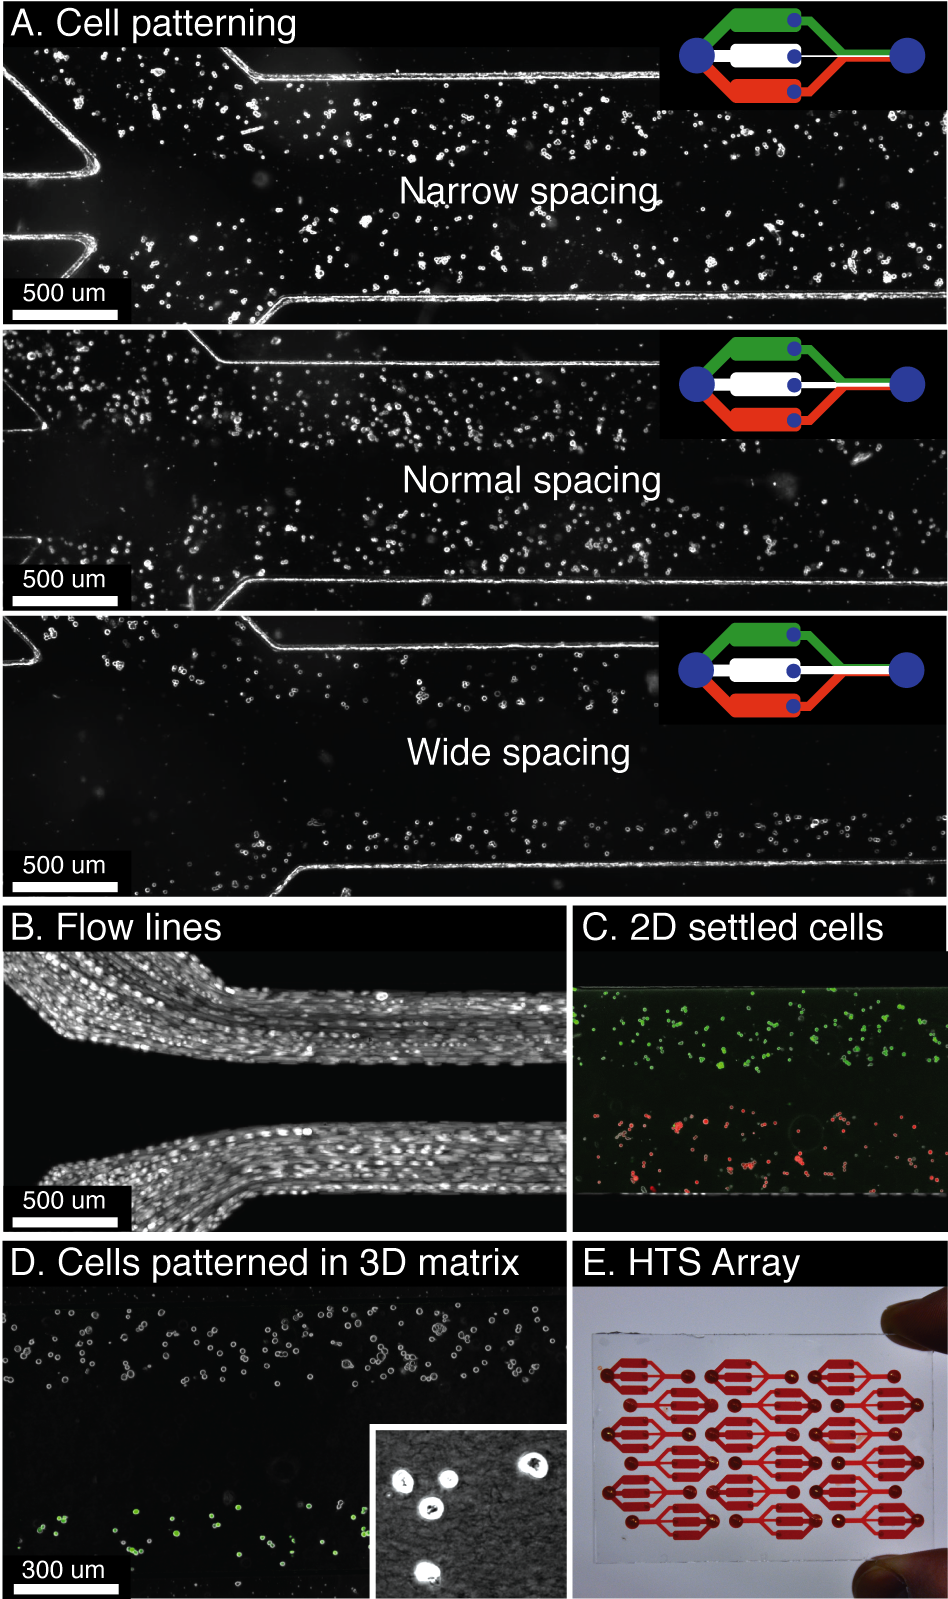
\includegraphics[width=8cm]{figure4.png}
  \caption{\textbf{Laminar flow patterning demonstrations}. A. Demonstration of a wound-healing/migration assay with variable spacing between the two cell populations. The upper right diagram represents the microfluidic device geometry. B. Multiple contrast enhanced movie-frames superimposed to illustrate the flow paths of cells being patterned in the wound-healing\slash migration device. C. RFP and GFP MCF7 cells patterned into a three-flow device. D. Osteoblasts (MC3T3-E1) and prostate cancer cells (LNCaP) are patterned within in a collagen matrix. The inset shows collagen fibers formed after polymerization using phase contrast imaging. E. Illustration of the arraying ability of the method for high-throughput screening (HTS) applications. All images  were taken within 15 min of seeding.} 
  \label{fig:experimental2}
\end{figure}

Fig \ref{fig:experimental2} illustrates the ability to scale the technique to incorporate more than two streams for 2-D or 3-D culture as well as for increased throughput and screening applications. Cell suspensions of MCF7 cells transfected with either GFP or RFP were patterned a set distance apart using a third stream of PBS directed down the center of the channel. In each case, only the width of the center branch was varied to produce a narrow (150 $\mu$m), medium (250 $\mu$m), and wide (600 $\mu$m) spacing (Fig \ref{fig:experimental2}A). Fig \ref{fig:experimental2}B is the superposition of multiple movie frames taken using phase contrast in order to illustrate the path of each cell in suspension as it travels. Fig \ref{fig:experimental2}C shows the final result of patterning using a false-colored overlay of the fluorescent images with an enhanced phase contrast image. Fig \ref{fig:experimental2}D demonstrates the ability to pattern cells in 3-D matrices such as collagen. As shown in Fig \ref{fig:experimental2}E, the individually addressable devices can be arrayed to enable inclusion of multiple experimental conditions on a single chip.

\subsection{Patterning for Cell-Based Assays}

%\subsection*{Discussion and Demonstration of Potential Applications}

The pipette-based strategy makes the method significantly more accessible to biologists by eliminating the need for syringes, tubes, and fluidic connections. The method is also more appropriate and robust for cell-based applications than other pipette-based methods which require the use of surface treatments and surfactants in the fluid to make patterning predictable \cite{Kim:2005fk}. As with other pipette-based methods, flow is transient and best-suited for applications where only a short period of flow is needed to establish the desired pattern, such as transient gradient generation, co-culture assays, wound-healing assays, and other particle patterning applications in 2-D or 3-D. Fig \ref{fig:cocultureData} illustrates the ability to use this method with cells to perform wound healing and co-culture assays.

%{\bf Generating Gradients.} Gradient generation is one of the most popular applications of LFP, and is used to study gradient sensing, chemotaxis and stem cell differentiation. Using passive pumping methods, transient gradients of factors are readily achievable by flowing two different media in the Y-channel (Fig. \ref{fig:gradient}). The gradient is initially steep at the boundary between the different fluids and eventually equilibrates. The time over which this occurs is given by Eq \ref{equ:transientGradient} with $D$ being the diffusion coefficient and  $L_{W}$ being the width of the channel. Longer term gradients can be achieved by subsequent applications of new drops at the loading ports to reset the gradient or through the use of a different pumping strategies. Nevertheless, transient gradients can be sufficient to study short term phenomena, such as the chemotaxis of rapidly migrating cells such as leukoctyes \cite{Berthier:2010uq}.

%\begin{equation}
%t = \frac{ L_{W}^{2} }{2D}
%\label{equ:transientGradient}
%\end{equation}

%\begin{figure}[!t]
%\centering
%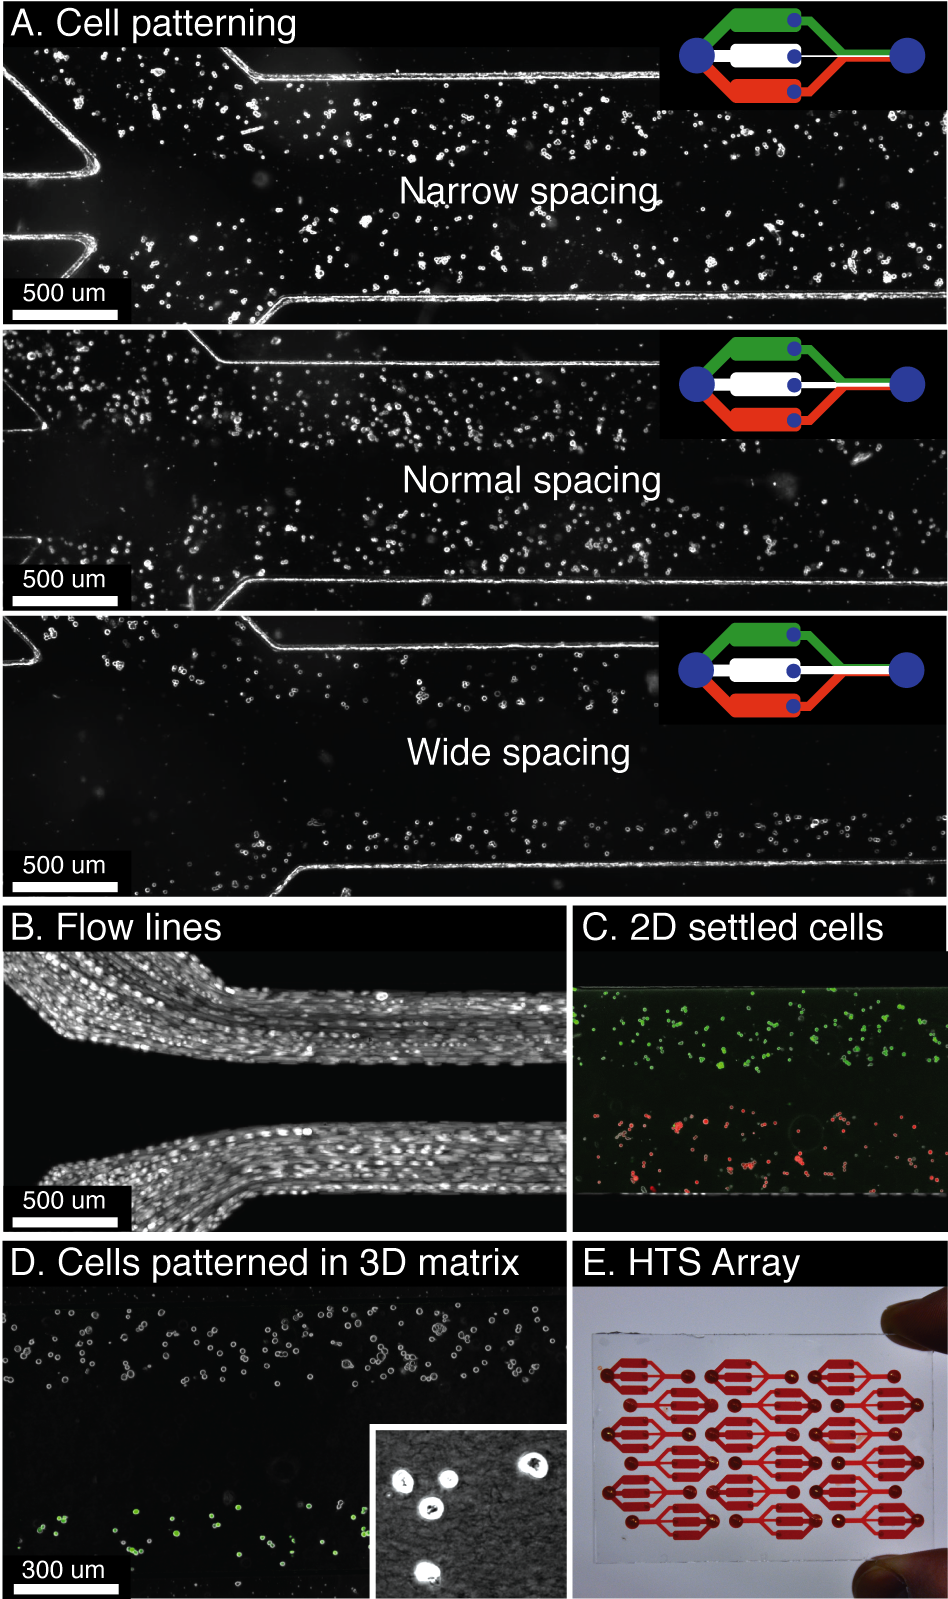
\includegraphics[width=8cm]{figure4.jpg}
%  \caption{Creation of a transient gradient using LFP of two different solutions.  }
%  \label{fig:gradient}
%\end{figure}



%A three-flow LFP devices (Fig \ref{fig:experimental2}) can be used to repeatably establish a gap between two cell populations for the study of soluble factor effects in co-culture and wound-healing\slash migration assays. The primary difference between these two types of assays is whether or not cells are allowed to migrate and close the gap. In a wound-healing/migration assay, closing of the gap is desired but can also result in cell-cell contact. In contrast, cell-cell contact can confound results in co-culture assays aimed at isolating soluble factor effects making it desirable to avoid cell migration in the region between the populations. This patterning method is flexible and can be used in conjunction with surface treatments or other culture channel geometries to avoid gap closure and prolong observation of soluble factor interactions. Although LFP has been used for these types of assays in the past, the method described here makes it significantly more accessible to a broader audience. In order to highlight some of the advantages of LFP for those that might now employ it in their application, a device for studying soluble factor interactions is demonstrated and compared to other more common methods of segregating cells, such as the use of constrictions or barriers.

The patterning technique was used with a lung epithelial cell line (BEAS-2B) to illustrate the potential for performing wound healing assays. Dotted lines show the initial patterning location and the advance of the cells onto the blank substrate in the center. Groups of cells form protrusions via collective migration instead of each cell migrating independently to advance the front uniformly (Fig \ref{fig:cocultureData}A, Day 2, white arrow). Fig \ref{fig:cocultureData}B illustrates the same patterning method with two different cell types, MC3T3-E1 and LNCaP, to demonstrate a directed cell migration or invasion assay. Given the channels are individually addressable without the use of valves or other microfluidic components, appropriate controls can be easily performed on the same array (i.e. blank+A, A+A, B+B, and blank+B). Similarly, different treatments can be applied to each channel at different time-points. A subtle, but important, capability of this method is the ability to change the cell ratio (i.e. 2 x A + B, or A + 3 x B) using different flow ratios (see Fig \ref{fig:experimental1}) while maintaining a constant surface cell density -- something that cannot be done in standard transwell assays \cite{Domenech:2009jt}. This ability can be crucial for controlling the confounding effects of density dependent cell behavior seen in many \emph{in vitro} models of cell signaling.
\begin{figure}[!t]
\centering
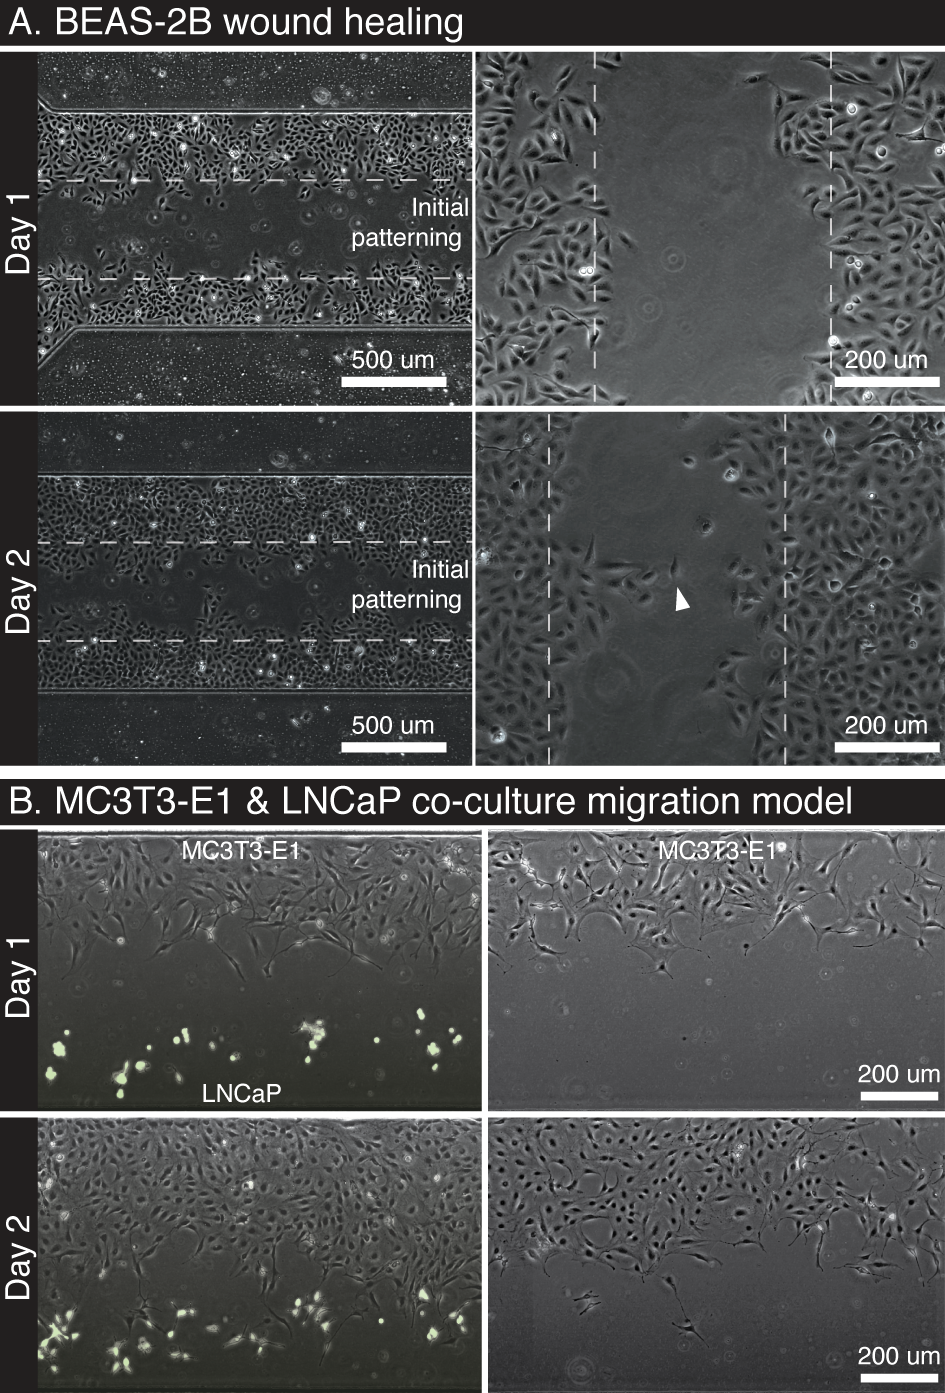
\includegraphics[width=3.2in]{figure5.png}
\caption{\textbf{Wound and migration assays}. A. Wound healing assay. BEAS-2B cells initially patterned with a defined gap and observed using phase-contrast over the course of 3 days. B. Migration assay. MC3T3-E1 and LNCaP (GFP$^{+}$, green) cells initially patterned with a gap to observe migration. A no-LNCaP control is provided within the same microchannel array as a control.}
\label{fig:cocultureData}
\end{figure}

This pipette-based approach offers multiple specific advantages for cell-based assays in addition to increased accessibility. Each channel is individually addressable allowing any number of fluids and cells suspensions to be loaded into a each channel of an array at any time without valving or changing fluidic connections. Arrays of the pipette-based devices can be addressed using liquid handling automation to increase throughput. Soft-lithography can be used to tailor the device geometry to change the ratio of one cell-type to another without changing the surface cell density. The distance between the groups of cells can be tuned to modulate soluble factor signaling to study soluble factor sensitivity. Additional branches can easily be added to create more complex co-culture assays containing more than two cell types. The device also supports the culture of cells in small volumes to enable more rapid accumulation of factors, a characteristic which has shown to improve co-culture sensitivity \cite{Domenech:2009jt}. Taken, together, the method offers significant advantages that increase the flexibility of the method and can broaden the use of LFP in cell-based assays.

%\begin{figure}[!t]
%\centering
%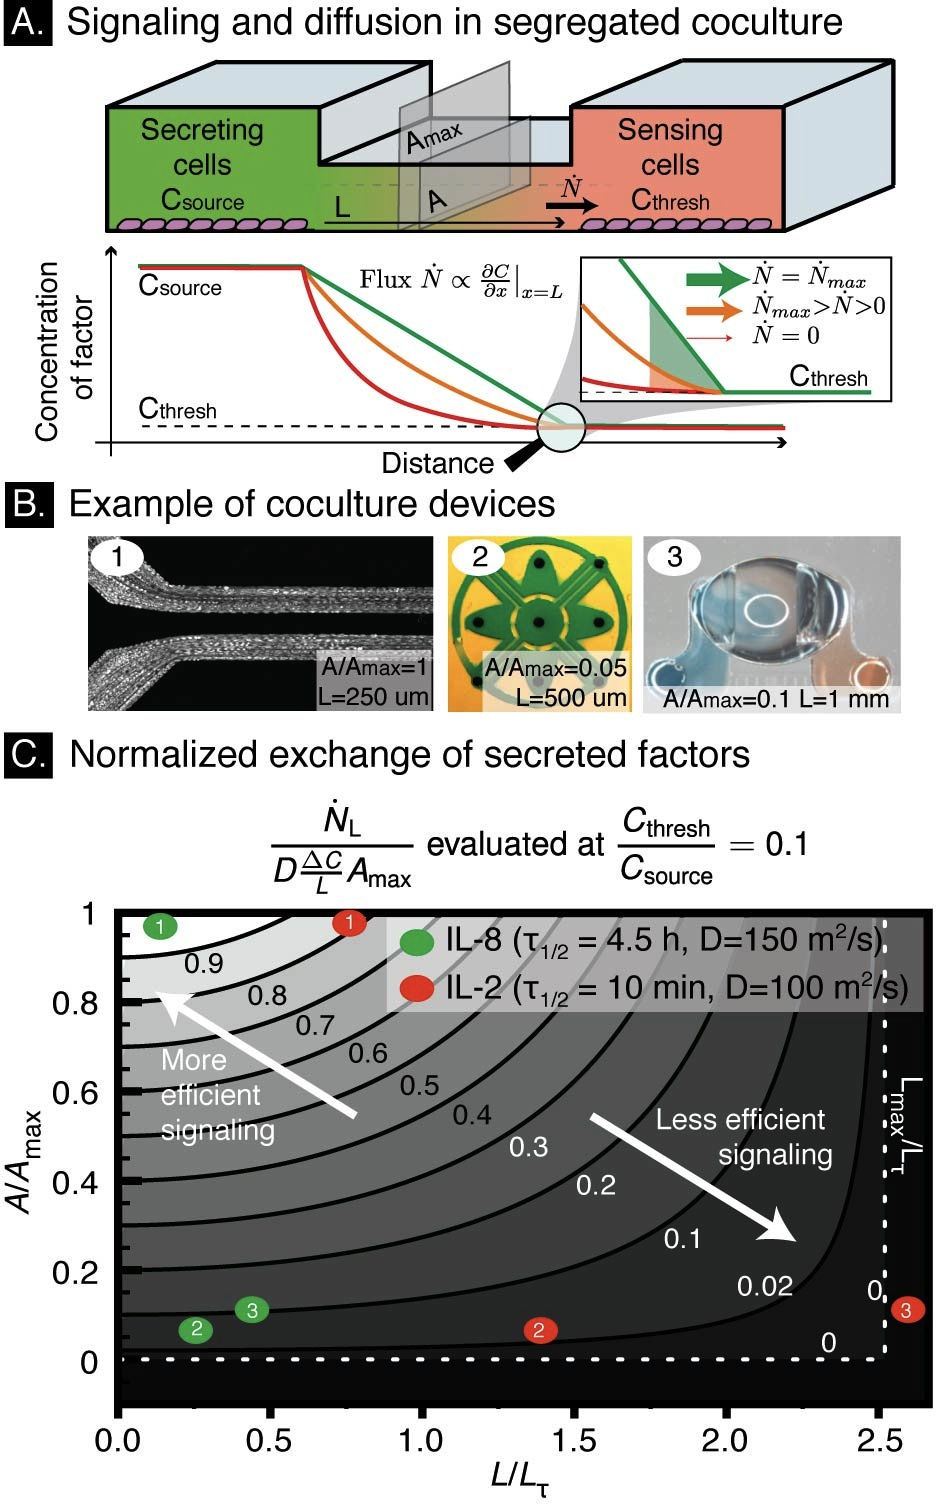
\includegraphics[width=3.2in]{figure6.jpg}
%\caption{Typical approaches for studying cell co-culture in a microchannel while keeping the cell cultures seperated. Laminar flow patterning provides the highest signaling ability as it maximizes diffusional exchange. Segregated co-culture provides simple sequential loading ability, though the flow-restricting constriction acts to limit signaling flux \cite{Domenech:2009jt}. Gel separated co-culture approach allows simple loading of the cell sample and usually higher signaling flux than segregated co-culture however fabrication and setup are more complex \cite{Sudo:2009fk}.}
%\label{fig:cocultureSchematic}
%\end{figure}

%Given the limited use of LFP for coculture and that many different devices and methods exist to perform segregated coculture, a qualitative analysis of diffusion between two cell populations is used to illustrate how LFP can be leveraged to improve soluble factor exchange. In a coculture assay, the groups of cells are typically separated by a gap through which factors must diffuse to initiate signaling. This basic scenario is illustrated in Fig \ref{fig:cocultureSchematic}. The three critical parameters that determine the efficacy of signaling between the populations are; $L$, the distance between the groups of cells; $D$, the diffusion coefficient; and $A$ the cross-sectional area through which the transport must occur. Using Fick's first law of diffusion, we can see that using constrictions to aid cell patterning acts to reduce the cross-sectional area for diffusion and thus diminish the rate of diffusive transport, $\dot{N}$ (Eq \ref{equ:ficks}, Fig. \ref{fig:cocultureSchematic}B). 
%\begin{equation}
%\dot{N} = D\,\frac{\partial C}{\partial x} A
%\label{equ:ficks}
%\end{equation}
%A similar effect is seen when the diffusion coefficient in the gap between the cells is lowered\cite{Domenech:2009jt}, for example with the use of gels or membranes as cell barriers \cite{Sudo:2009fk} (Fig \ref{fig:cocultureSchematic}C). The $\partial C/\partial x$ term suggests that culturing the cells in close proximity (\emph{i.e.}, by reducing $L$), helps to improve transport. Pipette-based LFP provides a way to implement coculture, wound-healing, and migration assays while avoiding the use of constrictions or barriers and enabling precise control of the distance between the each population to promote soluble factor signaling.

\section{Conclusions}

While LFP is an attractive method for studying cell migration, soluble factor signaling, and other biological phenomena, it has not been readily available for robust every-day-use in biology laboratories. The passive LFP method described here allows samples to be loaded at any time and in any order using only a pipette without depending on the use of syringes, tubes, fluidic connections, surface treatments, or surfactants. This advance enables the design and creation of practical assays that can leverage advantages of LFP to study soluble factor signaling and are amendable to use in biology labs. Furthermore, the synchronization method described here is compatible with patterning and in-situ polymerization of cell-laden hydrogels such as collagen or matrigel. These are increasingly gaining momentum as being central to the study of cell migration/invasion in three-dimensional matrices as they offer more physiologically relevant environments \cite{Sung:2010fk}.

\section{Acknowledgements}
David J. Beebe has an ownership interest in Bellbrook Labs LLC, which has licensed technology reported in this publication. The developments reported were accomplished through funding from the following grants: NIH-NCI R33 CA137673, DOD PCRP Idea (W81XWH-09-1-0192), Korea Research Foundation Grant (KRF-2008-220-D00133), a traineeship from the National Library of Medicine (5T15LM007359, J. Warrick) and a doctoral fellowship from the Morgridge Institute for Research (E. Berthier). We wish to thank Sameer Mathur for providing the BEAS-2B cells.